\documentclass{examen}

\begin{document}
\modulo{Lenguajes de marcas -- PARTE ESCRITA}

\pregunta{Crear en HTML un formulario como el mostrado en la figura}{2}
\begin{figure}[h]
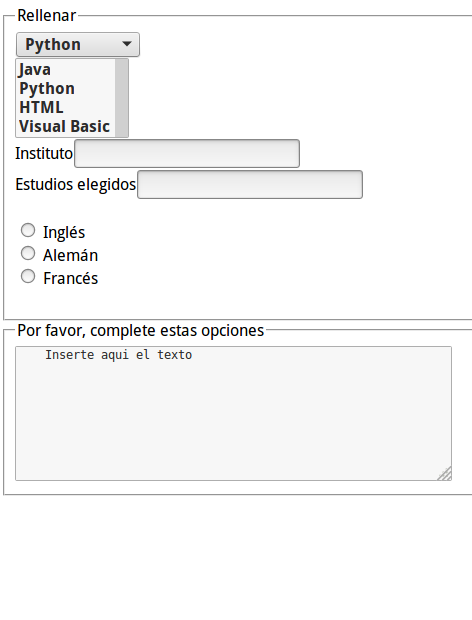
\includegraphics[scale=0.5]{examen-img/foto_formulario_11.png}
\end{figure}
\break

\pregunta{Repetir el mismo ejercicio anterior pero creando un esquema XML. Se repiten a continuaci�n los requisitos}{3}
\begin{itemize}
\item{    La ra�z se llama {\tt listafacturas}.}
\item{    Dentro de la lista debe haber uno o m�s elementos {\tt factura}.}
\item{    Las facturas tienen un atributo {\tt fecha} que es optativo.}
\item{    Toda factura tiene un {\tt emisor}, que es un elemento obligatorio y que debe tener un atributo {\tt cif} que es obligatorio. Dentro de {\tt emisor} debe haber un elemento {\tt nombre}, que es obligatorio y puede o no haber un elemento {\tt volumenventas}.}
\item{    Toda factura debe tener un elemento {\tt pagador}, el cual tiene exactamente la misma estructura que emisor.}
\item{    Toda factura tiene un elemento {\tt importe}.}
\end{itemize}

\begin{verbatim}
<!--Ejemplo de fichero-->
<listafacturas>
  <factura fecha="11-2-2017">
        <emisor cif="123">
          <nombre>ACME</nombre>
        </emisor>
        <pagador cif="234">
          <nombre>ACME Inc</nombre>
          <volumenventas>2000</volumenventas>
        </pagador>
        <importe>2500</importe>
  </factura>
</listafacturas>
\end{verbatim}
\end{document}
